\documentclass[12pt]{report}

\usepackage{amsmath} % for equations
\usepackage{graphicx} % for adding images
\usepackage[margin=1.0in]{geometry} % make margins smaller
\usepackage{listings} % for code blocks
\usepackage{hyperref} % for links
\usepackage{blindtext} % for Latin trash
\usepackage{setspace} % for line spacing
\usepackage{indentfirst}
\usepackage{titling}

\linespread{1.8}
%\doublespacing

\pretitle{\begin{center}\huge}
\posttitle{\par\end{center}\vspace{\baselineskip}}
\preauthor{\normalfont\normalsize\begin{center}\begin{tabular}[t]{c}}
\postauthor{\end{tabular}\end{center}\vspace{\baselineskip}}

\title{CSCE 465 Cryptography in Action}
\author{Nathan Brockway\\Dominick Fabian\\Blake Nelson}

\begin{document}
\maketitle

\newpage
\date{Submitted: December 8, 2018}
\maketitle

\tableofcontents
\newpage

\begin{abstract}
    Since as early as the ancient Roman days, secret messages have been sent from a command post to the front during wartime. With the constant risk of messengers being captured and their messages intercepted, a method of ensuring that only the authorized parties were able to read messages has been necessary. Such is the beginning of cryptography and the battle to devise new ways to break cryptographic systems. This project seeks to demonstrate the strengths and weaknesses in current popular cryptographic systems such as RSA, El Gamal, and DES. To do this, a client and a server are connected over the TCP/IP stack and exchange information. The client will send an encrypted message to the server, and the server will decrypt this and respond back with its own encrypted message. The client will then be able to decrypt and read this reply. Meanwhile, a malicious user will capture the encrypted communications en route and attempt to break the cryptographic system. To do this, a brute force and a more intelligent method will be used to recover the plaintext from the ciphertext. In this report, we analyze and discuss the performance of each of these attack vectors on a number of cryptosystems. Unsurprisingly, the brute force attacks on encryption are not nearly as effective as more sophisticated attacks that extort some of the weaker mathematical properties of the cryptosystems. These results are summarized in graphs and explained in depth in this report.
\end{abstract}

% for the progress report only
\iffalse
    \section{Task Assignments}
    \subsection{Write Symmetric Key Encryption}
    \begin{tabular}{l|l|l}
        Name & Assignee & Status \\ \hline
        DES & Blake & incomplete \\
        One Time Pad & Blake & incomplete	 
    \end{tabular}

    \subsection{Write Public Key Encryption}
    \begin{tabular}{l|l|l}
        Name & Assignee & Status \\ \hline
        RSA & Dominick & complete \\
        El Gamal & Nathan & complete
    \end{tabular}

    \subsection{Write Signature Protocols}
    \begin{tabular}{l|l|l}
        Name & Assignee & Status \\ \hline
        RSA & Dominick & complete \\
        El Gamal & Nathan & complete \\
        DSA & Nathan & incomplete	 
    \end{tabular}

    \subsection{Write Decryption Attacks}
    \begin{tabular}{l|l|l}
        Name & Assignee & Status \\ \hline
        RSA (Brute Force) & Dominick & complete \\
        RSA ($p-1$ factoring) & Dominick & complete \\
        El Gamal (Brute Force) & Nathan & incomplete \\
        El Gamal (Pollig-Hellman) & Nathan & incomplete \\
        El Gamal (Shank's) & Nathan & incomplete \\
        DES (Brute Force) & Blake & incomplete \\
        OTP (Brute Force) & Blake & incomplete 
    \end{tabular}

    \subsection{Implement Man-in-the-Middle Attacks}
    \begin{tabular}{l|l|l}
        Name & Assignee & Status \\ \hline
        Packet Sniffing & Blake & incomplete 
    \end{tabular}

    \subsection{Analyze Tasks}
    \begin{tabular}{l|l|l}
        Name & Assignee & Status \\ \hline
        Compare Private vs. Public Encryption & Blake & incomplete \\
        Compare Decryption Attack Methods & Nathan and Dom & incomplete
    \end{tabular}
\fi

% for the progress report only
\iffalse
    \section{Timeline}
    \begin{tabular}{l|l|l|l}
        Task & Assignee & Completion Date & Work Effort\\ \hline
        Develop Client/Server Framework & Blake & November 1 & 1 week\\
        Successfully Send Plaintext Message & Blake & November 15 & 2 days\\
        Complete RSA Encryption/Decryption & Dominick & November 25 & 1 day\\
        Complete El Gamal Encryption/Decryption & Nathan & November 25 & 1 day\\
        Complete DES Encryption/Decryption & Nathan & November 28 & 1 day\\
        Complete RSA Signature & Dominick & November 28 & 1 day\\
        Complete El Gamal Signature & Nathan & November 28 & 1 day\\
        Execute RSA Decryption Attack & Dominick & December 1 & 3 days\\
        Execute El Gamal Decryption Attack & Nathan & December 1 & 3 days\\
        Execute DES Decryption Attack & Blake & December 1 & 3 days\\
        Execute MITM Attacks & All Members & December 3 & 2 days\\
        Write Up Attack Successes/Failures & All Members & December 3 & 1 day\\
        Project Presentation & All Members & December 4/6\\ 
        Write Final Report & All Members & December 8 & 2 days
    \end{tabular}
\fi


\chapter{Final Report}
% for the progress report and the final report
\section{Introduction}
Mathematicians and computer scientists have spent years developing new algorithms that allow for the safe transfer of information from one party to another. These algorithms have come down to two main approaches: symmetric key encryption, where both parties share a single key used to encrypt and decrypt a message, and public key encryption, where both parties use a common key for encryption, but also have their own, private keys used in decryption. In our schooling, we have learned algorithms using both approaches, from both this class and MATH 470 - Communications and Cryptography. In this project, we will implement a few of these algorithms using Python and TCP sockets, and evaluate their effectiveness. We will first demonstrate the efficiency of the algorithm: how long it takes to get from plaintext to plaintext end to end compared to the length of the key. Next, we will use topics discussed previously in this class regarding packet sniffing to intercept and attempt to decrypt the message, using various methods discussed both in this class and previously in MATH 470. By timing both the message transfer and the ability to crack the decryption, we will put together a comprehensive study on the effectiveness of the algorithms individually and form a comparison between symmetric key encryption and public key encryption. Finally, we evaluate the efficiency and effectiveness of the Digital Signature Algorithm (DSA).

% for the progress report and the final report
\section{Background and Literature Review}
Both public and private key encryption have long histories.\cite{first-ten} Public key cryptography, specifically RSA and El Gamal, were conceived by cryptographers and mathematicians in the early 1970s.\cite{ieee}\cite{rsa} They were used by both the British and American government for over 20 years before finally being declassified and made public. A few years later, both algorithms were independently developed and published by their respective namesakes.

Meanwhile, symmetric key encryption was based on the One Time Pad encryption scheme, and the similarities are apparent, as many stream and block ciphers (two approaches to symmetric encryption) are based on each bit, or block, being used in an exclusive-OR operation. One Time Pad and block ciphers can be traced back to as early as 1949 when it was first proven to be secure. The Data Encryption Standard (DES) is a well known symmetric key algorithm, dating back to 1975 when it was first published, but there are more recent algorithms such as AES, published in 1998. This project will combine all of these into a comprehensive review of effectiveness and efficiency.

In addition to the need to keep messages secret while they are en route, there is a need to verify authenticity of a message. Verifying that a message was indeed sent from the person that they claim to be is arguably as important as sending the message itself. Very similar to one adding one's written signature to the bottom of a document to signify his or her agreement with the document, digital signatures work much the same way. This digital signature took the form of the Digital Signature Algorithm (DSA) in 1991 with support from the U.S. Government.\cite{mit}\cite{dsa}

\section{Method and Approach}
\subsection{Attacking RSA}
The strength of RSA comes from the idea that it is difficult to factor a large product of two primes. Since this has been deemed computationally infeasible, the security of the cryptosystem is based completely on this idea. This means that if $n$ can be factored, then RSA-encrypted communications are no longer secure. Before discussing the methods attempted to factor a product of two large primes, let us first understand why RSA relies on the secrecy of these prime factors.

As RSA is a public key cryptosystem, each user in the system has both a public and a private key. The public key is denoted $(e,n)$ and the private key is denoted $(d,n)$, where $n$ is the product of two large primes and $e,d$ are the encryption and decryption exponents, respectively. $n$ is made by multiplying two large primes, $p$ and $q$. Then the Euler totient of $n$, $\phi(n)$, is calculated as $\phi(n) = (p-1)(q-1)$. This is used to calculate $e$ and $d$ such that $ed \equiv 1$ (mod $\phi(n)$). Since $e$ and $n$ are made public to the whole world, finding $\phi(n)$ would allow anybody to calculate the decryption exponent and thereby both decrypt all communications encrypted with the corresponding public key and impersonate the holder of the private key. In order to calculate $\phi(n)$, the prime factors $p$ and $q$ need to be found. Thus, the idea that finding such factors of $n$ is difficult remains as the basis of the RSA cryptosystem.

The number of primes less than a given number $x$ can be approximated as $\frac{x}{ln(x)}$. If a 2048-bit RSA key were to be used, this number would have about 617 digits in base 10. This means that there are a \textbf{huge} number of potential prime numbers that could be factors of $x$ and it would take a \textbf{very} long time to try them all, even for a powerful computer.

For this project, two methods of factoring $n$ are explored: brute-force guessing and Pollard's $p-1$ method.\cite{pollard} Our brute force implementation takes the ultimate naive approach and simply tries every single odd number less than $n$ until it finds one of the factors. Once it finds one of the factors of $n$, it is trivial to find the other factor and $\phi(n)$ is easily calculated. By taking an inverse mod of $\phi(n)$ using the known encryption exponent, $e$, any ciphertext created with $d$ can now be decrypted.

Pollard's $p-1$ method takes a much more intelligent approach. Instead of trying to guess the correct answer, we start with $a=2$ and set a bound $B$ to be around 100 or so. Then we calculate $b=2^{B!}$ (mod $n$). If $gcd(b-1,n)$ is not 1 or $n$, then we have a non-trivial factor of $n$. If we do not get a non-trivial factor of $n$, we simply increase the size of our bound $B$ and try again. For larger key sizes, a larger $B$ must be used. Varying $a$ is also a valid approach to factorize $n$. The method works because of Fermat's Little Theorem, a very important theorem in number theory. Since $(p-1)|B!$, this implies that $B!$ is an integer multiple of $(p-1)$. From this, we see that
$b \equiv 2^{B!}$ (mod $p$) $\equiv 2^{k(p-1)}$ (mod $p$) $\equiv$ 1 (mod $p$)
and it is easy to get a prime factor from $p-1$ by adding 1. The bottleneck of the Pollard method is how quickly you can calculate $2^{B!}$ (mod $p$) since the factorial makes the amount of computation grow at beyond exponential rates!

For a comparison of the two attacks on RSA, section \ref{results}.

\subsection{Attacking El Gamal}
Just as RSA relies on the computational infeasibility of factoring products of large primes, El Gamal relies on what is known as the Discrete Logarithm Problem. The premise of this problem is that given the congruence $a^{x} \equiv b$ (mod $n$) and that $n$ is prime, for some known $a^{x}$, $b$, and $n$ there is no efficient way to find $x$. However, there are still some methods of recovering a plaintext from an El Gamal ciphertext of various effectiveness. For this project, we experiment with brute-force, the Pollig-Hellman method, and the Shank's method. 

shanks rainbow, pollig breaks the one big time of shanks into a bunch of smaller ones

\subsection{Attacking DSA}
birthday attacks

\subsection{Attacking DES}
DES is a symmetric key algorithm designed in 1975 in conjunction with the U.S. Government. While no longer considered to be a safe algorithm for sensitive information, its popularity in past years makes it worthwhile to attack and benchmark. DES takes in a 64-bit key and uses this key to create 16 sub-keys to be used in each round of the DES encryption. The algorithm was designed to be easy to implement in hardware and difficult to implement in software, so this proved a bit of a challenge to design in our Python scripts and is going to be significantly slower running in software than it would be using actual DES hardware.

For this project, we experiment with a brute force attack on DES. To do this, we first need a known plaintext/ciphertext pair. Once we have this, we continually generate a random set of keys, encrypt the plaintext, and check to see if the result is the ciphertext. If we get the ciphertext from the pair as a result, then we have found the key needed to generate the DES key sets.

\subsection{Attacking One-Time Pad}
I think you can literally only try brute force attacks on this...

\section{Results}
\label{results}

\begin{figure}[hp!] % [hp!] means ''here''
    \begin{center}
        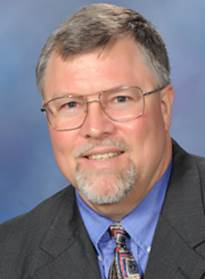
\includegraphics[width=0.5\linewidth]{walker.jpg}
        \caption{Comparison of Brute-Force and $p-1$ Attacks on RSA}
        \label{fig:rsa}
    \end{center}
\end{figure}

\begin{figure}[hp!] % [hp!] means ''here''
    \begin{center}
        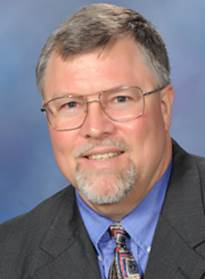
\includegraphics[width=0.5\linewidth]{walker.jpg}
        \caption{Comparison of Attacks on El Gamal}
        \label{fig:el-gamal}
    \end{center}
\end{figure}

\section{Discussion and Recommendations}

\section{Conclusion}
deez nuts

% an example bibliography
\newpage

\begin{thebibliography}{9}

    \bibitem{first-ten}
    The First Ten Years of Public-Key Cryptography\\
    \texttt{https://cr.yp.to/bib/1988/diffie.pdf}
    
    \bibitem{ieee}
    A Public Key Cryptosystem and a Signature Scheme Based on Discrete Logarithms.\\
    \texttt{https://ieeexplore.ieee.org/document/1057074/}

    \bibitem{rsa}
    A Method for Obtaining Digital Signatures and Public-Key Cryptosystems\\
    \texttt{https://people.csail.mit.edu/rivest/Rsapaper.pdf}
    
    \bibitem{philzimmerman}
    Why I Wrote PGP.\\
    \texttt{https://www.philzimmermann.com/EN/essays/WhyIWrotePGP.html}
    
    \bibitem{stanford}
    The Diffie Hellman Problem.\\
    \texttt{https://crypto.stanford.edu/~dabo/pubs/papers/DDH.pdf}
    
    \bibitem{mit}
    A Method for Obtaining Digital Signatures and Public Key Cryptosystems.\\
    \texttt{https://people.csail.mit.edu/rivest/Rsapaper.pdf}

    \bibitem{pollard}
    Notes on Pollard's $p-1$ Attack on RSA\\
    \texttt{https://www.math.columbia.edu/~goldfeld/PollardAttack.pdf}

    \bibitem{dsa}
    Digital Signature Standard (DSS)\\
    \texttt{https://web.archive.org/web/20131226115544/http://csrc.nist.gov/\\publications/fips/fips1861.pdf}

\end{thebibliography}

\newpage
\section{Appendix A: Source Code}
All of the source code for this project can be found at:

\href{https://github.com/NelsonBlakeN/CryptoInAction}{https://github.com/NelsonBlakeN/CryptoInAction}.

\newpage
\section{Appendix B: Presentation Slides}

\end{document}
